\renewcommand{\tool}{WASM-MUTATE\xspace}
\msection{\tool: Fast and Effective Binary for WebAssembly}

In this section, we introduce our third technical contribution, \tool \cite{wasmmutate}, a tool that generates thousands of functionally equivalent variants out of a WebAssembly binary input. 
Leveraging rewriting rules and e-graphs \cite{e-graph} for software diversification, \tool synthesizes program variants by transforming parts of the original binary. 
In \autoref{fig:approach_landscape}, we highlight \tool as the blue squared tooling.

\begin{figure*}[h!]
    \centering
    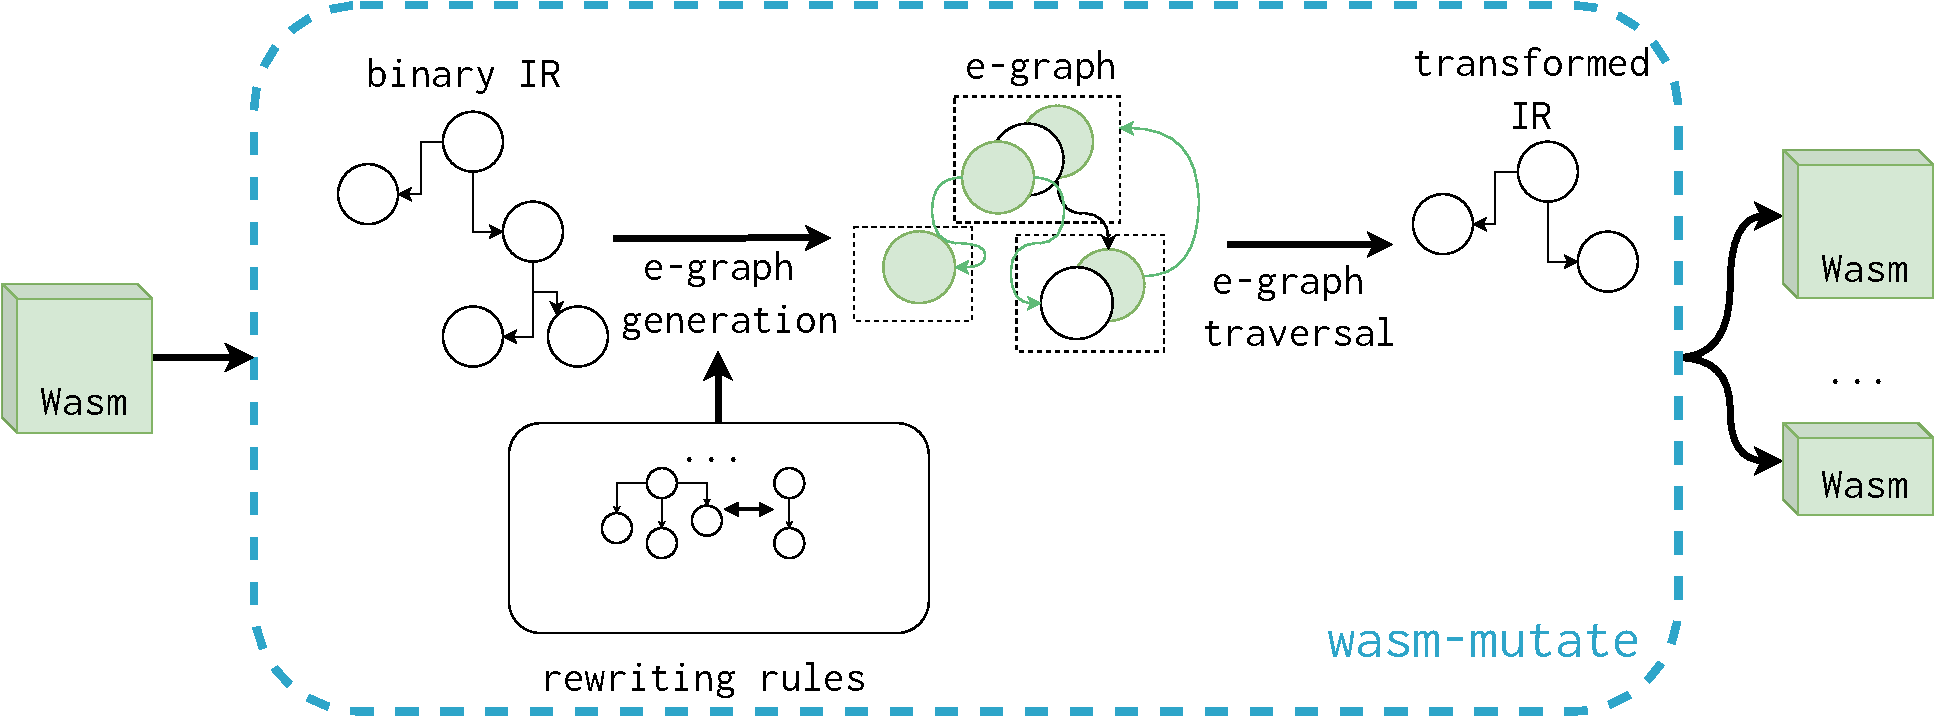
\includegraphics[width=0.9\linewidth]{diagrams/wasm_mutate.workflow.pdf}
    \caption{ \tool high-level architecture.  It generates functionally equivalent variants from a given WebAssembly binary input. 
    Its central approach involves synthesizing these variants by substituting parts of the original binary using rewriting rules, boosted by diversification space traversals using e-graphs.}
  \label{fig:wasm-mutate}
\end{figure*}


\autoref{fig:wasm-mutate} illustrates the workflow of \tool, which initiates with a WebAssembly binary as its input. 
The first step involves parsing this binary to create suitable abstractions, e.g. an intermediate representation.
Subsequently, \tool utilizes predefined rewriting rules to construct an e-graph for the initial program, encapsulating all potential equivalent codes derived from the rewriting rules. 
The assurance of functional equivalence is rooted in the inherent properties of the individual rewrite rules employed.
Then, pieces of the original program are randomly substituted by the result of random e-graph traversals, resulting in a variant that maintains functional equivalence to the original binary. 
\tool applies one transformation at a time.
The output of one applied transformation can be chained again as an input \Wasm binary, enabling the generation of many variants.


\msubsection{WebAssembly Rewriting Rules}
\label{custom}

\tool contains a comprehensive set of 135 rewriting rules.
In this context, a rewriting rule is a tuple \texttt{(LHS, RHS, Cond)} where \texttt{LHS} specifies the segment of binary targeted for replacement, \texttt{RHS} describes its functionally equivalent substitute, and \texttt{Cond} outlines the conditions that must be met for the replacement to take place, e.g. enhancing type constraints.
\tool groups these rewriting rules into meta-rules depending on their target inside a \wasm binary, ranging from high-level changes affecting binary section structure to low-level modifications within the code section. 
This section focuses on the biggest meta-rule implemented in \tool, the \texttt{Peephole} meta-rule \footnote{For an in-depth explanation of the remaining meta-rules, refer to \cite{wasmmutate}.}. 

% Determinism
Rewriting rules inside the \emph{Peephole} meta-rule, operate over the data flow graph of instructions within a function body, representing the lowest level of rewriting.  
In \tool, we have implemented 125 rewriting rules specifically for this category, each one avoiding targeting instructions that might induce undefined behavior, e.g., function calls.

% Augmentation of the internal representation
Moreover, we augment the internal representation of a \wasm program to bolster \tool's transformation capabilities through the \texttt{Peephole} meta-rule.
Concretely, we augment the parsing stage in \tool by including custom operator instructions.
These custom operator instructions are designed to use well-established code diversification techniques through rewriting rules.
In practice, custom operators are only part of the rewriting rules of WASM-MUTATE.
This means that, when parsing Wasm to the intermediate representation no custom operator is generated.
When converting back to the \Wasm binary format from the intermediate representation, custom instructions are meticulously handled to retain the original functionality of the \Wasm program. 
Remarkably, custom operators highlight the versatility of \tool as a general-purpose binary rewriting engine.


In the example below, we illustrate a rewriting rule of the \texttt{Peephole} meta-rule that leverages a custom operator to insert \texttt{nop} instructions into any \Wasm program place, a well-known low-level diversification strategy \cite{homescu2013profile}, while using the \texttt{container} custom operator.
When generating the \wasm variant, the \texttt{container} custom operator is removed while its operands are encoded back to Wasm in their corresponding opcodes.
\begin{minipage}{0.9\linewidth} 
    
\lstdefinestyle{watcode}{
    numbers=none,
    stepnumber=1,
    numbersep=10pt,
    tabsize=4,
    showspaces=false,
    breaklines=true, 
    showstringspaces=false,
      moredelim=**[is][{\btHL[fill=black!10]}]{`}{`},
      moredelim=**[is][{\btHL[fill=celadon!40]}]{!}{!}
  }
  
  {
  \captionsetup{width=\linewidth}
  \noindent\begin{minipage}[b]{\linewidth}
      \lstset{
          language=ttt,
          style=watcode,
          basicstyle=\footnotesize\ttfamily,
          columns=fullflexible,
          breaklines=true}
          \begin{lstlisting}[]{Name}
   LHS x
          \end{lstlisting}
          %\vspace{0.2cm}
     \end{minipage}
     
  \noindent\hrulefill
  
  \noindent\begin{minipage}[b]{\linewidth}
      \lstset{
          language=ttt,
          style=watcode,
          basicstyle=\footnotesize\ttfamily,
          columns=fullflexible,
          breaklines=true}
          \begin{lstlisting}[]{Name}
   RHS (container (x nop))
          \end{lstlisting}
          %\vspace{0.2cm}
     \end{minipage}
     
  }
  
\end{minipage}



\msubsection{E-Graphs traversals}


We developed \tool leveraging e-graphs, a specific graph data structure for representing and applying rewriting rules \cite{10.1145/3571207}. 
In the context of \tool, a primer e-graph is constructed from the input \Wasm program.
This initial e-graph is subsequently augmented with e-nodes and e-classes derived from each one of the rewriting rules (we detail the e-graph construction process in Section 3 of \cite{wasmmutate}).

% General use of case
Willsey et al. highlight the potential for high flexibility in extracting code fragments from e-graphs, a process that can be recursively orchestrated through a cost function applied to e-nodes and their respective operands.
This methodology ensures the functional equivalence of the derived code \cite{e-graph}. 
For instance, e-graphs solve the problem of providing the best code out of several optimization rules \cite{10.1145/1480881.1480915}.
To extract the "optimal" code from an e-graph, one might commence the extraction at a specific e-node, subsequently selecting the AST with the minimal size from the available options within the corresponding e-class's operands.
In \too omitting the cost function from the extraction strategy leads us to a significant property: \emph{any path navigated through the e-graph yields a functionally equivalent code variant}. 

We exploit such property to fastly generate diverse \Wasm variants.
We propose and implement an algorithm that facilitates the random traversal of an e-graph to yield functionally equivalent program variants, as detailed in \autoref{peephole:mutator}. 
This algorithm operates by taking an e-graph, an e-class node (starting with the root's e-class), and a parameter specifying the maximum extraction depth of the expression, to prevent infinite recursion.
Within the algorithm, a random e-node is chosen from the e-class (as seen in lines 5 and 6), setting the stage for a recursive continuation with the offspring of the selected e-node (refer to line 8). 
Once the depth parameter reaches zero, the algorithm extracts the most concise expression available within the current e-class (line 3). 
Following this, the subexpressions are built (line 10) for each child node, culminating in the return of the complete expression (line 11).


\algnewcommand\algorithmicforeach{\textbf{for each}}
\algdef{S}[FOR]{ForEach}[1]{\algorithmicforeach\ #1\ \algorithmicdo}
\begin{algorithm}
    %\footnotesize
	\begin{algorithmic}[1]
	%	\Procedure{MyProcedure}{}
      \Procedure{traverse}{$egraph$, $eclass$, $depth$}
        \If{depth = 0}
          \State  \Return \textbf{smallest\_tree\_from}(egraph,\ eclass)
        \Else
            \State $nodes \gets egraph[eclass]$
            \State $node \gets random\_choice(nodes)$
            \State $expr \gets (node, operands=[])$
            \ForEach {$child \in node.children $}
                \State $subexpr \gets \textbf{TRAVERSE}(egraph,\ child,\ depth - 1)$
                \State $expr.operands \gets expr.operands \cup\ \{subexpr\}$
            \EndFor
            \State \Return $expr$
        \EndIf
        \EndProcedure
	\end{algorithmic} 
	\caption{e-graph traversal algorithm taken from \cite{wasmmutate}.} 
	\label{peephole:mutator}
\end{algorithm}



\msubsection{\tool instantiation}

% \todo{FIX cross refs}

% Example of a random e-graph traversal 
Let us illustrate how \tool generates variant programs by using the before enunciated algorithm.
Here, we use Algorithm \ref{peephole:mutator} with a maximum depth of 1.
In \autoref{example:peeporig} a hypothetical original Wasm binary is illustrated.
In this context, a potential user has set two pivotal rewriting rules: \texttt{(x, container (x nop),)} and \texttt{(x, x i32.add 0, x instanceof i32)}.
The former rule, which has been previously discussed in \autoref{custom}, grants the ability to append a \texttt{nop} instruction to any subexpression. 
Conversely, the latter rule adds zero to any numeric value .



\begin{minipage}[b]{\linewidth}
    \lstset{
        language=WAT,
                        style=watcode,
        basicstyle=\footnotesize\ttfamily,
                        columns=fullflexible,
                        breaklines=true}
        
        \begin{lstlisting}[label=example:peepapplied,caption={Random peephole mutation using e-graph traversal for \autoref{example:peeporig} over e-graph \autoref{e-graph3}. The textual format is folded for better understanding.},frame=b, captionpos=b]{Name}
(module
    (type (;0;) (func (param i32 f32) (result i64)))
    (func (;0;) (type 0) (param i32 f32) (result i64)
        !(i64.add (!
            !i64.const 0!
            !i64.const 1!
            !nop!
        !))!
    )
        \end{lstlisting}
\end{minipage}

\end{minipage}



\begin{figure}
    \centering
    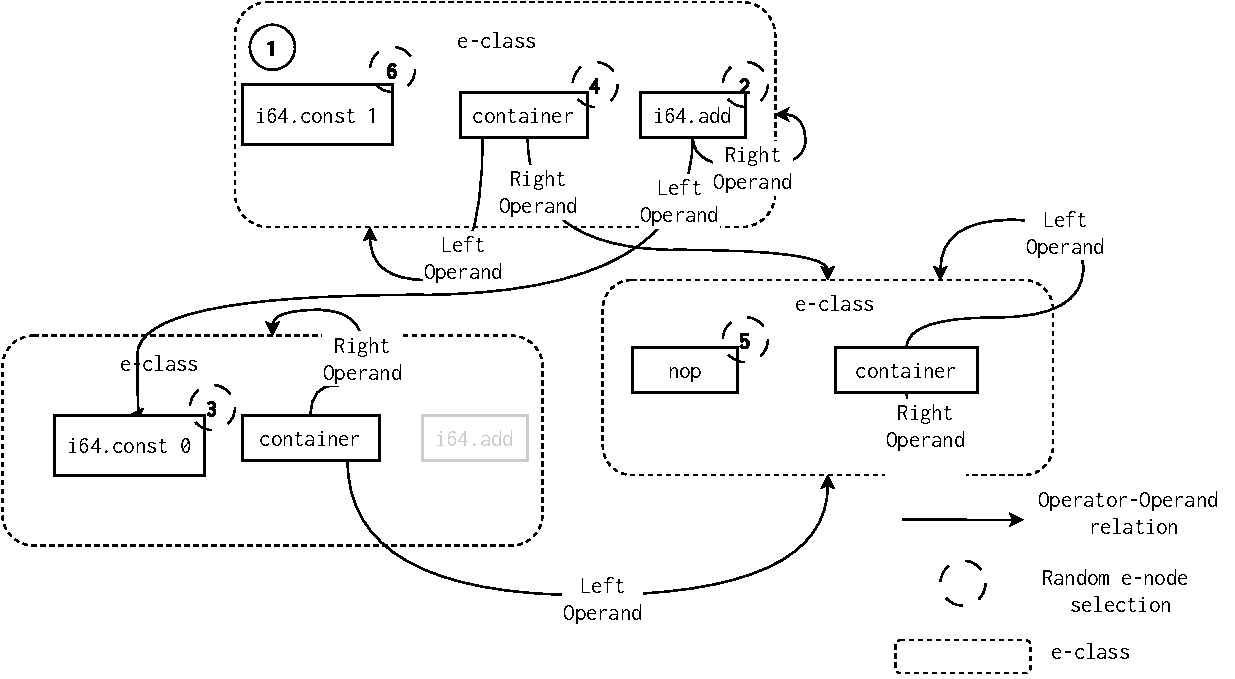
\includegraphics[width=1.0\linewidth]{figures/e-graph-traversal2.pdf}
    \caption{e-graph built for rewriting the first instruction of \autoref{example:peeporig}. }
  \label{e-graph3}
\end{figure}



Leveraging the code presented in \autoref{example:peeporig} alongside the defined rewriting rules, we build the e-graph, simplified in \autoref{e-graph3}.
In the figure, we highlight various stages of Algorithm \ref{peephole:mutator} in the context of the scenario previously described. 
The algorithm initiates at the e-class with the instruction \texttt{i64.const 1}, as seen in \autoref{example:peeporig}.
At \step{2}, it randomly selects an equivalent node within the e-class, in this instance taking the \texttt{i64.add} node, resulting: {\texttt{expr = i64.add l r}}.
As the traversal advances, it follows on the left operand of the previously chosen node, settling on the \texttt{i64.const 0} node within the same e-class \step{3}.
Then, the right operand of the \texttt{i64.add} node is choosen, selecting the \texttt{container} \step{4} operator yielding:
{\texttt{expr = i64.or (i64.const 0 container ( r nop ))}}.
The algorithm chooses the right operand of the \texttt{container} \step{5}, which correlates to the initial instruction e-node highlighted in \step{6}, culminating in the final expression:
{\texttt{expr = i64.or (i64.const 0 container( i64.const 1 nop))\ i64.const 1}}.
As we proceed to the encoding phases, the \texttt{container} operator is ignored as a real Wasm instruction, finally resulting in the program in \autoref{example:peepapplied}.

Notice that, within the e-graph showcased in \autoref{e-graph3}, the container node maintains equivalence across all e-classes. 
Consequently, increasing the depth parameter in \autoref{peephole:mutator} would potentially escalate the number of viable variants infinitely.

%s\todo{Augment this last paragraph.}


\begin{tcolorbox}[title=Contribution paper and artifact,boxrule=1pt,arc=.2em,boxsep=1.0mm]
  \tool leverages random traversals over e-graphs to provide a binary-based solution for \Wasm diversification. \\
  \tool is fully presented in Cabrera-Arteaga \etal "WASM-MUTATE: Fast and Effective Binary Diversification for WebAssembly"
 \url{https://arxiv.org/pdf/2309.07638.pdf}.
  \\\\
  \tool is available at \url{https://github.com/bytecodealliance/wasm-tools/tree/main/crates/wasm-mutate} as a contribution to the bytecodealliance organization \toolcite{https://bytecodealliance.org/}.
\end{tcolorbox}